%!TEX root=../report.tex

\section{Foundations}


Simulations are a \textit{problem-based discipline that allows for repeated testing of a hypothesis.} \cite{sokolowski2010modelingintro} This statement covers two important aspects of simulations in general. The first key element in this statement is \textit{“problem-based”}. This means a simulation always addresses a question. The second key element is \textit{“repeated testing”}. This means a simulation is intended to run multiple times.

The general approach to simulate something is to build a model as an abstraction of a system in the real world and then modify and observe the model according to the hypothesis that needs to be tested. The last step is to draw a conclusion out of the observations.

\subsection{Terminology}

System and model are widely used. To clarify their meaning in this report I explain their meaning in the context of simulations.

\subsubsection{System}

A model is intended to represent a system in the real world. Therefore the abstract term \textit{system} must be defined. In the scope of this report, a system is a collection of different elements that influence the simulation. This includes among other people, hardware, software, institutions, documents, and environmental factors. A system can be physically present in the real world, but it could also be a plan or concept for something that does not exist.


\subsubsection{Model}

The concept \textit{model} is a physical, mathematical, or otherwise logical
representation of a system. Models serve as representations of events and things. The events can be real, e.g. from an observation of the real world, or contrived. A model represents a system.
While a system could be dangerous to observe or even don't exist, a model could be used to study the evolution of a system. When investigating a system, a quantitative assessment is derived. This may include how the system performs with various inputs and in different environments.
Different scenarios (occurrence of specific events) can be investigated.  It is important to get a quantitative evaluation of the performance of the system. The performance could cover multiple aspects, which depend on the purpose of the model.
A model exists at three levels of abstraction: conceptual, specification, and computational. \cite[chapter 1]{leemis2006discrete} A conceptual model abstracts the general concept while a specification model contains concrete information. A computational model refers to an implemented program of a model, which means that the computational model is nothing else than a simulation. In this report computational model and simulation are equivalent. The classifications for simulations are also classifications of models.

In the following, I will go into more detail regarding different types of simulations, followed by a detailed explanation of discrete-event simulation, and lastly, introduce the cycle of modeling \& simulation.


\subsection{Classification of Simulations}


Simulations in general can be classified depending on multiple aspects. In this section, I will introduce a few approaches to classify simulations.

\subsubsection{Static \& Dynamic}

A system model is static or dynamic. A static model is one in which time
is not a significant variable. A dynamic model evolves over time. \cite{leemis2006discrete} \note{(chapter 1)}

Static models can answer the question of how much money gets distributed if \textit{N} people play the lottery next week. The result is completely independent of the timing of the players.
To solve such questions, there is the Monte Carlo simulation, that relies on repeated random sampling to obtain numerical results. Another use case for Mone-Carlo simulations is finding the area under a curve. \cite{ohriner1971finding}

If the system evolves over time it is a so-called dynamic model. A dynamic model would emerge if the lottery example gets extended by players that play week for week. Their spendings on the lottery could depend on their last result.


\subsubsection{Continuous \& Discrete}

A dynamic system model is continuous or discrete. Continuous simulations are based on a continuous function of time. Examples of continuous simulations can be found in classical mechanics. Examples are oscillating pendulums or a block sliding on an inclined plane. In each of these cases, the motion is characterized by one or more differential equations that model the continuous-time evolution of the system.
In contrast, discrete simulations are based on events that occur at discrete points in time. Only events can lead to a change in the system. Examples are inventory systems or board games.
An inventory system changes its state every time a new order arrives or new products arrive. These changes are not continuous, but they occur at a certain point in time.
The next section focuses on discrete-event simulation in more detail.

\begin{figure}[h!]
 \caption{Chosing the right simulation paradigm depending on the model requirements (adopted from \cite[page 3]{leemis2006discrete})}
 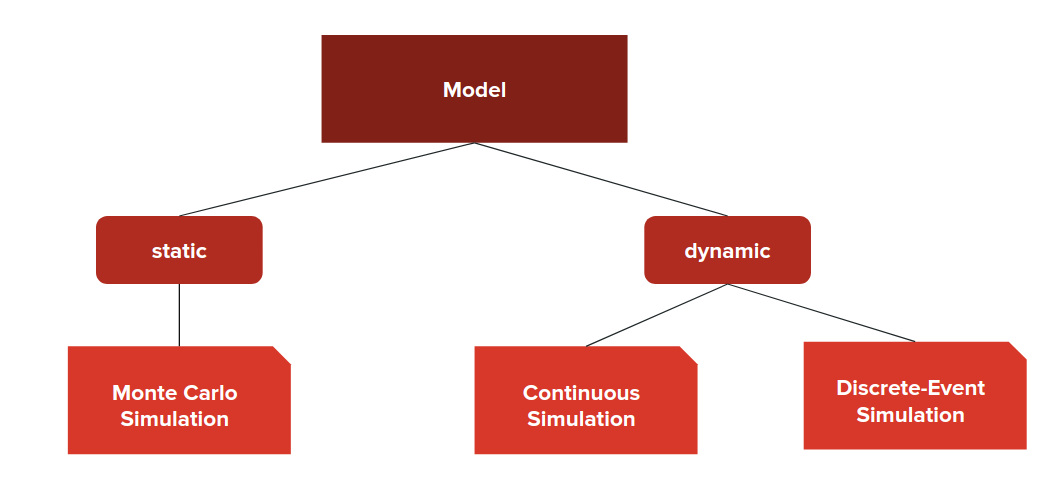
\includegraphics[width=0.9\textwidth]{static-dynamic-classification}
\end{figure}


\subsubsection{Fidelity, Resolution \& Scale}

There are three primary attributes that can be mapped to models or simulations.
These are fidelity, resolution, and scale. \cite{sokolowski2010modelingintro}

\textbf{Fidelity} indicates how close a simulation matches reality. A model that closely behaves like a real system has high fidelity. High fidelity means that every aspect of the system must be covered. Normally models aim to describe only the parts that are necessary for the initial hypothesis. Aiming for a high fidelity would mean a great effort. It should only be done if the hypothesis requires a high fidelity of the simulation.


\textbf{Resolution} describes the level of details. The more detail included in the simulation, the
higher the resolution. To illustrate this, a model of a plantation could be broken down into models of all single plants. Modeling all plants would achieve a higher resolution. The target resolution depends on the intention of the model. Referring to the plantation example, a model that should describe harvesting around the globe, would better use a low resolution, namely models of plantations, while a model to optimize the crop would need a higher resolution.

\textbf{Scale} indicates the overall size of the simulation. A larger system has a higher scale. The scale is a fairly subjective metric. It always depends on the relations. One example is simulating a fabric compared to simulating a single device in a production line.


\subsubsection{Games, Simulation Games \& Simulators}


Nearly every system can be simulated. In this report, I would like to have a deeper look into the field of games. Games play a popular role in the entertainment industry. There is a wide range of games that aim to simulate a system in an interactive way. These can be distinguished whether they aim for fun or for training.
Games, simulation games, and simulators can be distinguished based on various characteristics. \cite{narayanasamy2006distinguishing} In this scope \textit{games} mainly refers to computer games. But the characteristics also apply for board games.
All (computer) games have a simulation part somehow, but one characteristic is that simulation games do not always involve a specific goal-oriented activity within the context of the game. Games and simulation games aim for fun and entertainment. They provide challenges and have typical game patterns. The world can be imaginative or fictitious.
Simulators are designed for training. Training simulators only provide a real-world environment. They aim for skill-development rather than fun. Challenges in training simulators are challenges with equivalents in the real-world.



\subsection{Discrete-Event Simulation}

There are certain characteristics that define a discrete event simulation.
First of all, there must be a stochastic component. This means the state of our model depends on probabilities. At least one variable that defines the current state of the system must be random.
Secondly, the model is dynamic. This means, there is a change over time.
Thirdly, the changes of the model depend on discrete-events. These discrete-events can occur randomly at discrete time instances.


\begin{figure}[h!]
 \caption{Visualization of a discrete-event simulation system}
 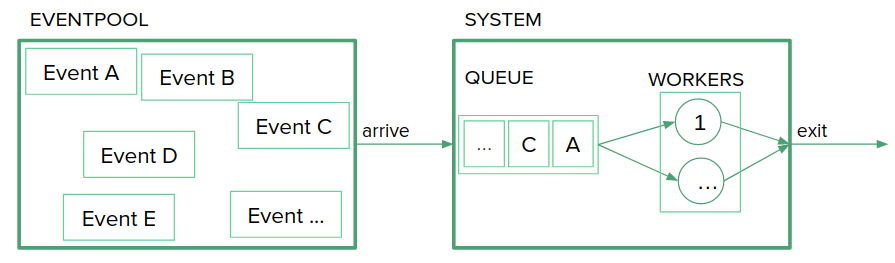
\includegraphics[width=0.9\textwidth]{queue-model}
\end{figure}

To visualize a discrete-event simulation, it can be seen as a queuing system. There are certain events that can occur and a system contains queue and workers that handle the events.
Depending on the scenario events are also called jobs or customers. Workers also have synonyms like server. The queue is sometimes renamed to \textit{event list} or \textit{calendar}. And the system is also called \textit{service node} in other literature.
Events arrive at the system at random points in time and each event could take a different amount of time to get processed by a worker before the event it can exit the system. The systems operate as follows: If a new event arrives, it will be moved into the queue. If the queue is not empty and at least one worker is not busy, one event is taken from the queue and gets processed.

From this behavior, two important terms regarding the timing can be derived.
Delay. The delay is the time that an event remains in the queue. the delay is greater or equals zero.
Wait. The wait for an event is the duration between arrival and exit. In other words, the wait is the delay plus the processing time of the worker.

Reducing delay and wait is a common optimization goal that discrete-event simulation can be used for. This could be achieved by adding more workers or changing the way how events are selected from the queue. A common technique is FIFO (first in, first out) that always takes the event with the greatest delay. Other techniques try to optimize the delay by prioritizing events with a small processing time (also known as \textit{shortest job first}).

\subsubsection{Components}
\label{des:components}

There are some main components that a discrete event simulation requires.

The System State. This captures all variables that characterize the simulation.

The Simulation Clock. This is a tool that tracks the elapsed time. Different approaches to increment the simulation clock are explained in \hyperref[des:timeadvance]{\textit{Time-Advance Mechanism}}.

Next - Event List. This is a queue for the upcoming events.

Statistical Counter or Accumulator. This is a tool that records the evolution of the system state.
%
%The initialization program is the setup method of the game class.
%
%
%The event subprogram is in the simulate function of the game class. In pseudo code the simulate functions runs in a loop till the game is finished. And we call the player.play function that modifies the current game state. This function contains all the logic to play the game. In my implementation it’s pick a card with the same color or same number otherwise take a card from the draw pile.
%
%The event subprogram is in the simulate function of the game class. In pseudo code the simulate functions runs in a loop till the game is finished. And we call the player.play function that modifies the current game state. This function contains all the logic to play the game. In my implementation it’s pick a card with the same color or same number otherwise take a card from the draw pile
%.

%
%(5) Initialization Subprogram. A protocol utilized in the initialization of
%the simulation, usually setting the start time to zero.
%(6) Timing Subprogram. A protocol that, drawing from a next - event list,
%sets the next event and progresses the simulation clock to the moment
%when an event is to happen.
%(7) Event Subprogram. A protocol that launches a routine that updates
%the state of the system with the occurrence of each event.
%(8) Library Subprogram. A protocol used to produce random observa-
%tions drawn generally from predetermined probability distributions.
%(9) Report Generator. A tool that calculates and reports statistics that
%describe the performance of the system.
%(10) Main Program. A routine that coordinates the concert of subordinate
%routines, executing these in the correct sequence. It initializes the
%timing subprogram that determines the subsequent event, passes
%control to the related event subprogram, and updates the system state.
%This routine verifi es for termination and triggers the report generator
%once the simulation ends.
%


\subsubsection{Trace-Driven Discrete-Event Simulation}

The events in a discrete-event simulation can be generated or prerecorded. If the simulation relies on prerecorded data, it is a so-called trace-driven discrete-event simulation.
By definition, a trace-driven simulation relies on input data from an external source to generate realistic events. \cite{leemis2006discrete} The advantage of trace-driven discrete-event simulations is that no data needs to be generated and the data source reveals realistic data. On the other hand, the reliance on external data limits the capabilities to simulate new scenarios. A common question is "What if \textit{X}" happens. And if \textit{X} not part of the recorded data it is not possible to find out.


\subsubsection{Next-Event Simulation}

The concept of next-event simulation extends the basic concept of discrete-event simulations. To construct a next-event simulation model, all events must be assignable to an event type. An algorithm decides how the system state changes depending on these event types.
\cite[chapter 5]{leemis2006discrete}
The algorithm for a next-event simulation is based on four steps.
\textbf{Initialization.} In this The simulation clock is initialized (usually to zero) and the first events get queued.
\textbf{Processing the current event.} The queue is scanned to determine the next event. Then the event gets processed the event and the simulation clock advances.
\textbf{Schedule new events}. New events (if any) that may be spawned by the current event are placed in the queue.
\textbf{Terminate}. The process of advancing the simulation clock and processing events and scheduling new events continues until some terminal condition is satisfied. The terminal condition can be a specific event that only occurs once. Another terminal condition could be reaching a certain time on the simulation clock.


\subsubsection{Time-Advance Mechanism}
\label{des:timeadvance}

The progress of time in a simulation is a very essential aspect. In discrete-event simulations, there are two well-known approaches: Fixed-increment advance and next-event time advance.
The fixed-increment advance initializes at time zero and advances at fixed time increments. The disadvantage is that events occur not in sync with the increments. This means the arrival time and exit time is probably not exact. Another characteristic of the fixed-increment advance is that the size of the time increment is subjective. But choosing the increment interval has implications for the performance measures of the system. Large increments lead to imprecise timing of the events, while small increments could lead to a situation where no changes happen for many increments.
In contrast, the next-event time-advance approach is more versatile. It initializes the simulation clock at zero and then progresses to the next upcoming event. The incrementation step is not fixed, but always in sync with the arrivals and exits of all events. This solves the disadvantages of the fixed-increment advance.



% \note{Using Queues is a useful concept since we have queues everywhere in the real world. For example, if you order at an online shop your delivery gets processed at many    If you travel, you have to wait for your bus or your plane.}


\subsection{Modelling \& Simulation Cycle}

\begin{figure}[h!]
 \caption{Process of generating and evaluating simulations (adopted from \cite[page \note{X}]{sokolowski2010modeling})}
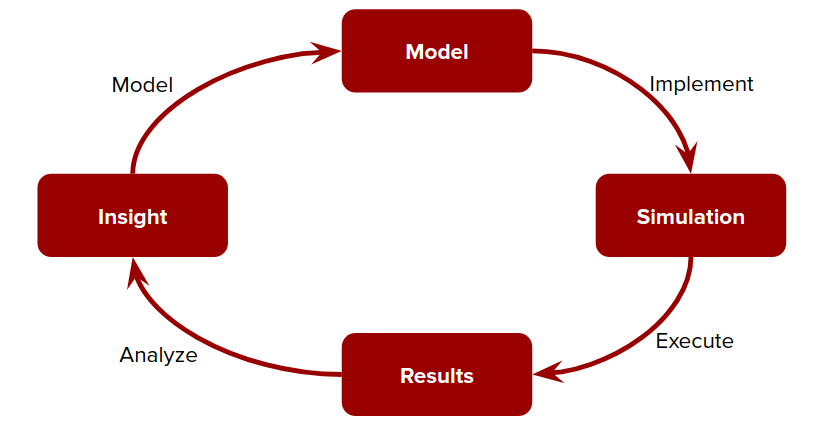
\includegraphics[width=0.9\textwidth]{simulation-modelling-cycle}
\end{figure}

Simulations are based on models and simulations are designed to answer a hypothesis. This means simulations must also be understood as a piece a larger process.
%The process of modeling and simulation is proposed by \note{Name}.
It starts with modeling. Modeling includes theories, information, algorithms of the topic. A decision must be taken which type of model and with paradigms are used. A supporting tool for that is the decision tree in \note{figure X}.
The result of the first phase is a model. The model gets implemented in the next step. There is dedicated software for simulation purposes. \cite{wiki:deslist} The result of this step is an executable program that implements the model.
During the execution phase, the simulation program generates data. For the execution, the processing environment must be taken into account. Complex simulations may need more computation power than a normal home computer could provide.
The output data must be transformed to get the desired performance insights.
If the model contains variability and uncertainty, then techniques from probability
and statistics will likely be required for the analysis. All further analysis must happen regarding the initial hypothesis. A model must be verified and validated. This means to check whether the model was built correctly and whether the model is appropriate compared to the real world.
 It is very likely that the results reveal that the model must be adjusted or extended. This means to reiterate through this cycle. It is a good practice to repeat the cycle as often as needed.

I will go through this cycle with an example of a discrete-event simulation use case in the next chapter.


